\chapter{Convolutional Neural Networks (CNNs)}

\space

\section{Motivation}

\textbf{Fully connected networks become useless when the dataset is not nicely preprocessed, centered, etc}. When the size of the input is incompatible with the dimensions of the model, the fully connected will no longer work because it needs to be retrained.\\

\\\textbf{Using a large fully connected network has some downsides}:
\begin{itemize}
    \item \textbf{Computation complexity (exponentially) grows} $\rightarrow$ harder to train
    \item \textbf{Larger capacity} $\rightarrow$ more data to generalize
    \item \textbf{Bad inductive bias} $\rightarrow$ Ignores geometry of image data (relative distances between objects in an image)
    \begin{itemize}
        \item Recall that in fully connected networks, the pixels of an image are stacked to make a line of pixels (1D) instead of a 2D image
    \end{itemize}
    \item \textbf{Not flexible} $\rightarrow$ Different image sizes require different models
    \begin{itemize}
        \item When we want to put a new image size as input in a model, we need to train the model from scratch
    \end{itemize}
\end{itemize}

\section{Convolution Operator}

\begin{definition}
    \textbf{Convolution:} Convolution is a mathematical operation on two functions f and g that expresses how
the shape of one is modified by the other. The function f is the input function and the function g is known as the\textbf{ kernel}.

\[
(f * g)(t) = \sum_{\tau = -\infty}^{\infty} f(\tau) \cdot g(t - \tau)
\]

\end{definition}

\begin{figure} [h!t]
    \centering
    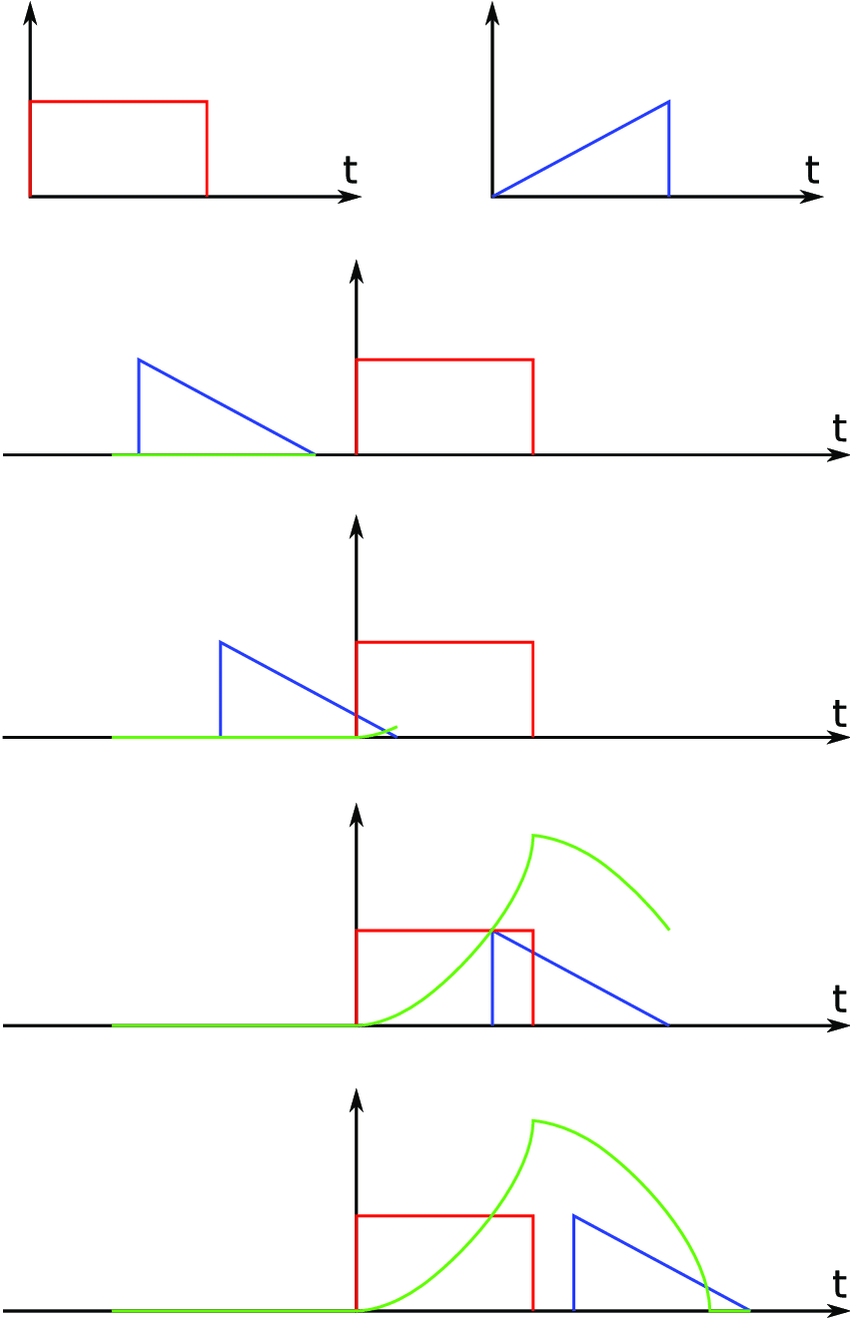
\includegraphics[width=0.27\linewidth]{convolution.png}
    \caption{Convolution}
    \label{fig:enter-label}
\end{figure}

\section{Convolution in 2D for Images}

To apply the convolutional operator to 2D space, we simply \textbf{add another dimension} to the equation.\\

\\\textbf{Convolution of Image \( I \) with filter kernel \( K \):}
\begin{enumerate}
    \item Multiply each pixel in the range of the kernel by the corresponding element of the kernel.
    \item Sum all these products and write the result to a new 2D array.
    \item Slide the kernel across all areas of the image until you reach the image's edges.
    \item Once the edge is reached, go back horizontally to the start but slide down one pixel
\end{enumerate}


\[y[m,n] = I[m,n] * K[m,n = \sum_{j=-\infty}^{\infty} \sum_{j=-\infty}^{\infty} I[i,j]\cdot K[m-i, n-j]\] 
\begin{figure}[h!t]
    \centering
    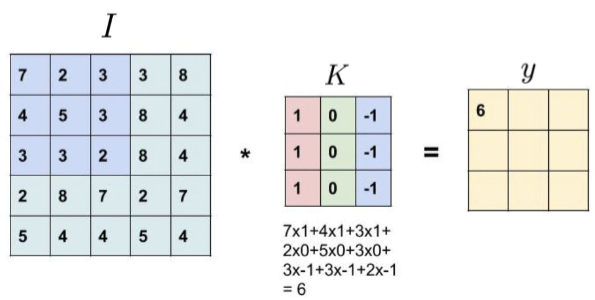
\includegraphics[width=0.5\linewidth]{convex1.png}
    \caption{Step 1}
    \label{fig:enter-label}
\end{figure}

\begin{figure}[h!t]
    \centering
    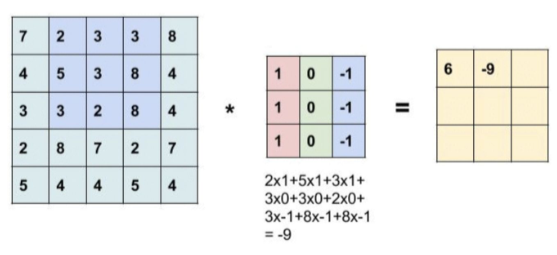
\includegraphics[width=0.525\linewidth]{convex2.png}
    \caption{Step 2}
    \label{fig:enter-label}
\end{figure}

\begin{idea}
    Convolution of an image is applying a kernel to the image while sliding the kernel across the image
\end{idea}


\textbf{Why use convolution?}
\begin{itemize}
    \item In signal processing, convolution is used to \textbf{extract important features} of the input signal
    \item Instead of trying to make prediction directly on image pixels, such as what we've done in fully connected networks, we are applying a kernel to the image pixels to extract interesting features, then do predictions based on those features (which are the most important assets of the image)
    \item The output of the kernel applied to the image is the most important assets of the image extracted by the kernel\\
\end{itemize}

\begin{definition}
    \textbf{Kernel:} a kernel, also known as a filter, is a small matrix used to extract specific features from an input image or data. It's applied through the process of convolution to scan the input and produce feature maps that highlight particular patterns, such as edges, textures, or other relevant characteristics. 
\end{definition}

\noindent\textbf{Examples of kernels (filters) applied to images}

\begin{itemize}
    \item \textbf{Blurring:} averages out pixel intensities in an image
    \begin{figure}[h!t]
        \centering
        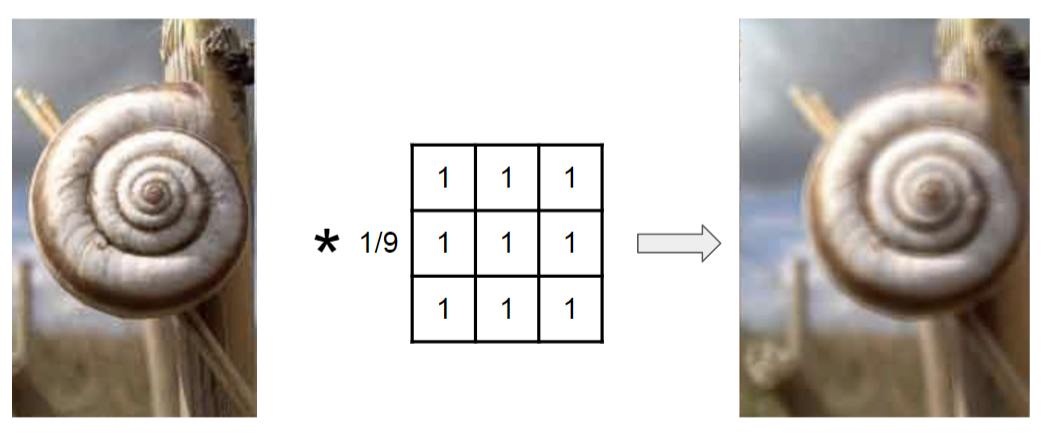
\includegraphics[width=0.45\linewidth]{blurringkernel.png}
        \caption{Blurring Filter}
        \label{fig:enter-label}
    \end{figure}
    \item \textbf{Vertical Edge Detector}
\begin{figure}[h!t]
    \centering
    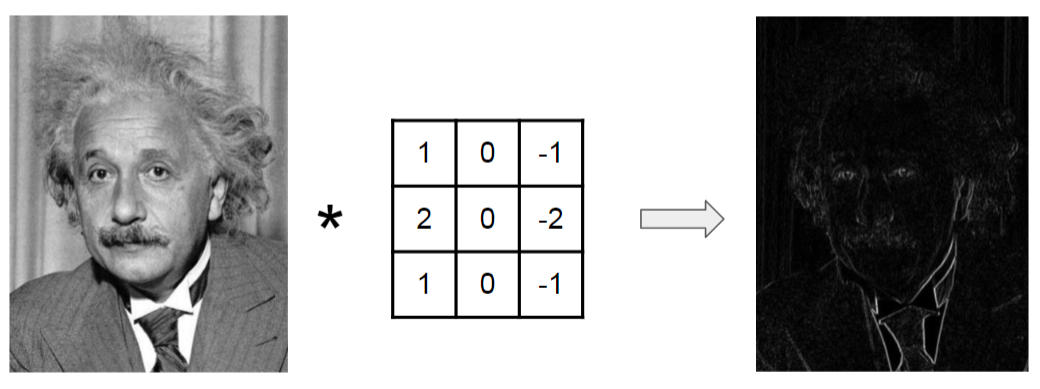
\includegraphics[width=0.45\linewidth]{verticaledgekernel.png}
    \caption{Vertical Edge Detector}
    \label{fig:enter-label}
\end{figure}
    \item \textbf{Horizontal Edge Detector}
\begin{figure}[h!t]
    \centering
    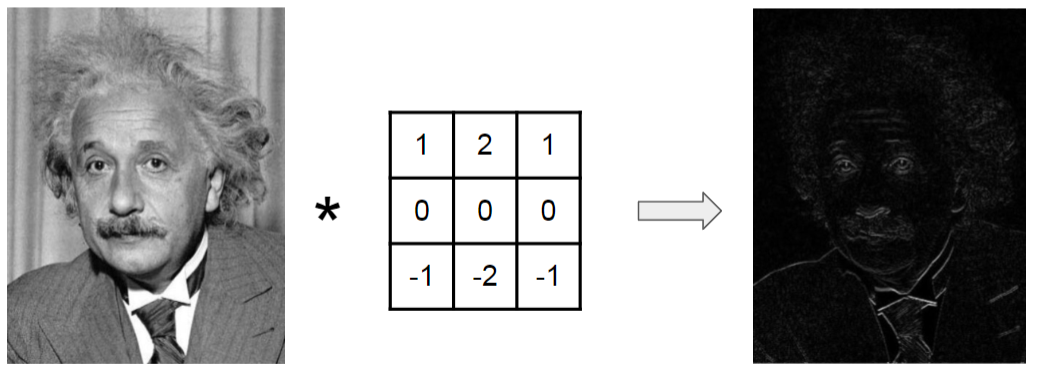
\includegraphics[width=0.45\linewidth]{horizontaledgekernel.png}
    \caption{Horizonal Edge Detector}
    \label{fig:enter-label}
\end{figure}
    \item \textbf{Blob Detector:} detect regions that differ in properties, such as brightness or color, compared to
surrounding regions
\begin{figure}[h!t]
    \centering
    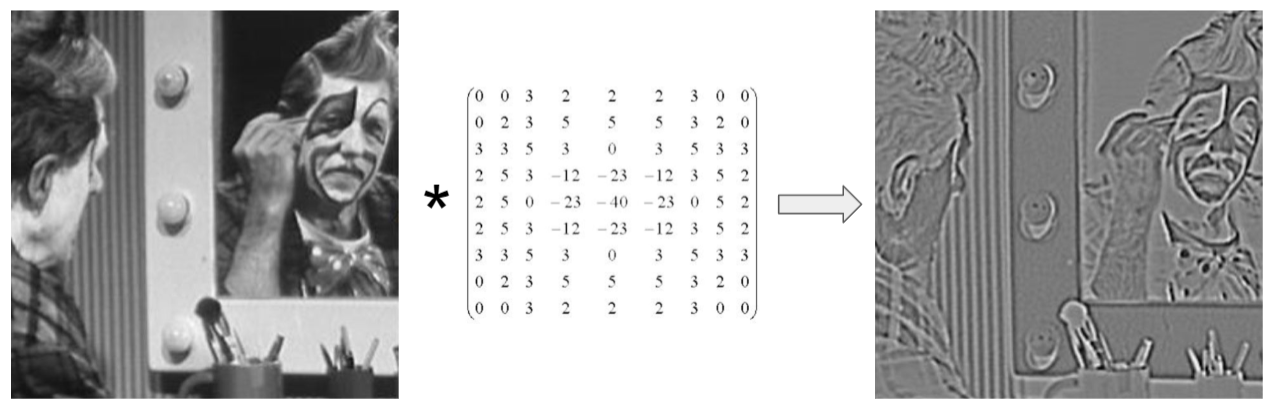
\includegraphics[width=0.45\linewidth]{blobdetectorkernel.png}
    \caption{Blob Detector}
    \label{fig:enter-label}
\end{figure}
\end{itemize}

\textbf{Where do these kernels come from?}

\begin{itemize}
    \item Before deep learning, people would spend years coming up with these kernels (hand-crafted)
    \item Classic computer vision used multi-stage feature (kernel) engineering
\end{itemize}

\begin{figure}[h!t]
    \centering
    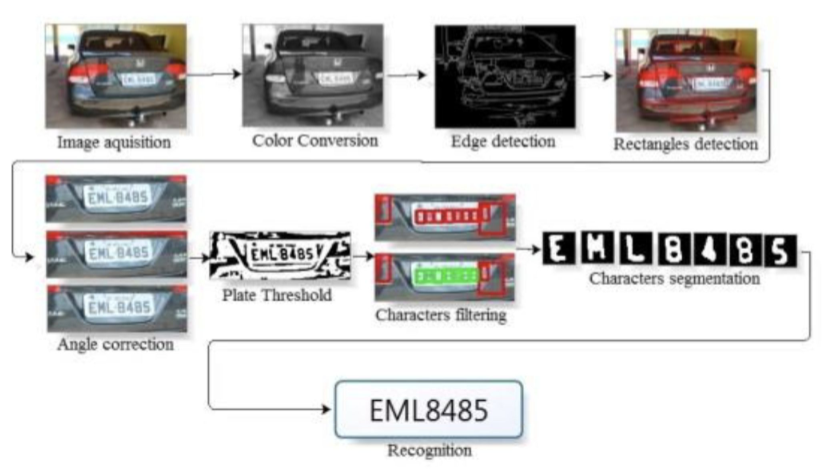
\includegraphics[width=0.5\linewidth]{multistagekerneleng.png}
    \caption{Multi-stage feature (kernel) engineering of a licence plate recognition system}
    \label{fig:enter-label}
\end{figure}

\begin{itemize}
    \item There were two main problems with this method:
    \begin{enumerate}
        \item If one step fails, the subsequent steps wil also fail
        \item Hand-written algorithms don't work in real world scenarios due to fringe cases
    \end{enumerate}
\end{itemize}
\begin{itemize}
    \item This is where convolutional neural networks become useful
\end{itemize}

\section{Convolutional Neural Networks}

\begin{definition}
    \textbf{Convolutional Neural Network:} a type of deep learning model specifically designed for processing and analyzing grid-like data, such as images and sequences. It uses layers of learnable filters (kernels) to perform convolutions on the input data, enabling the network to automatically learn and extract hierarchical features. CNNs are highly effective for tasks like image recognition, object detection, and image generation due to their ability to capture local patterns and spatial relationships within the data.
\end{definition}

Convolutional neural networks were\textbf{ inspired by the Hubel and Wiesel Cat Experiments (1958-1959)}:
\begin{itemize}
    \item Individual neurons respond to stimuli only in a restricted region of the visual field
known as the \textbf{Receptive Field}.
\item Collection of such fields overlap to cover the entire visual area
\item Some neurons react only to images of horizontal lines, while others react line
orientations
\item Higher-level neurons are based on the outputs of neighbouring lower-level
neurons


\end{itemize}

\textbf{Introduce convolutional filters into neural networks so that we don’t have to hand
craft the features!}
\begin{itemize}
    \item \textbf{Locally connected layers}: local features in small regions of the image
    \item \textbf{Weight sharing:} detect the same local features across the entire image
    \item Neural Network \textbf{learns the kernel values} (or weights)
    \item More efficient than fully-connected networks since \textbf{outputs of kernels are connected to neurons} instead of each individual pixel of an image (weight sharing). 
    \item \textbf{Detecting:} the output (activation) is high if the feature is present
    \item \textbf{Feature:} something in the image, like an edge, blob, or shape
    

\end{itemize}

\begin{figure}[h!t]
    \centering
    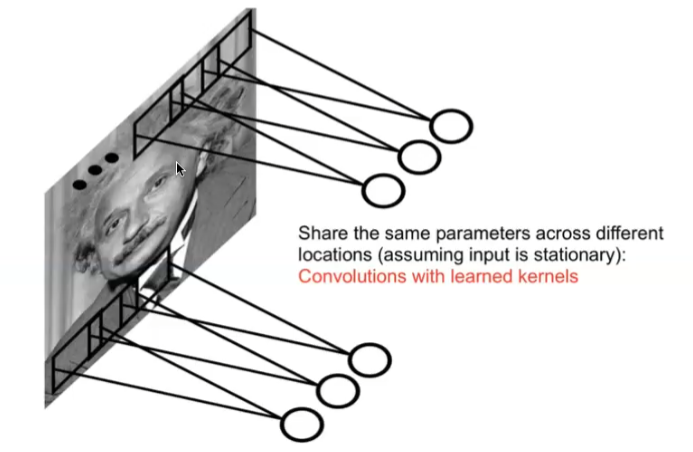
\includegraphics[width=0.3\linewidth]{weightsharing.png}
    \caption{Weight Sharing}
    \label{fig:enter-label}
\end{figure}



\begin{figure}[h!t]
    \centering
    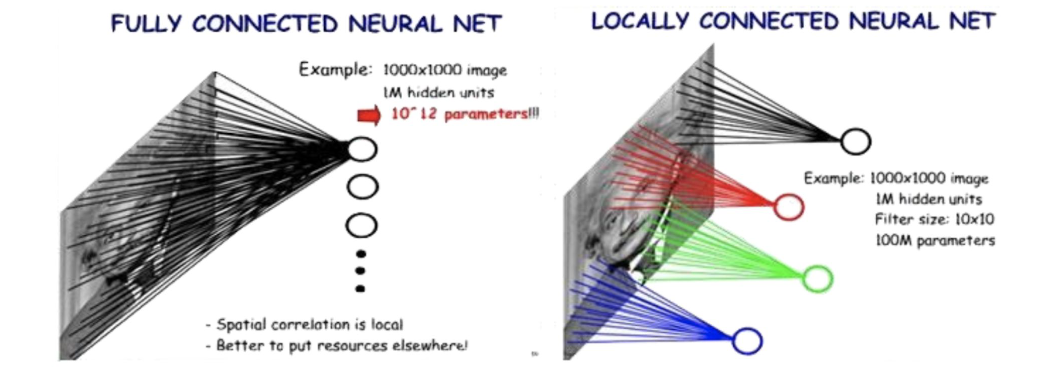
\includegraphics[width=0.5\linewidth]{fcvsconv.png}
    \caption{Fully Connected vs. Convolutional}
    \label{fig:enter-label}
\end{figure}

\newpage

While fully-connected networks require us to preprocess the input,

\begin{figure}[h!t]
    \centering
    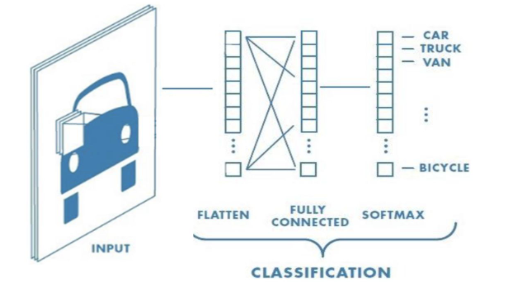
\includegraphics[width=0.35\linewidth]{fc.png}
    \caption{Fully connected network}
    \label{fig:enter-label}
\end{figure}

convolutional neural networks apply convolution to image tensors and allow the network to learn and extract important low and high level features.

\begin{figure}[h!t]
    \centering
    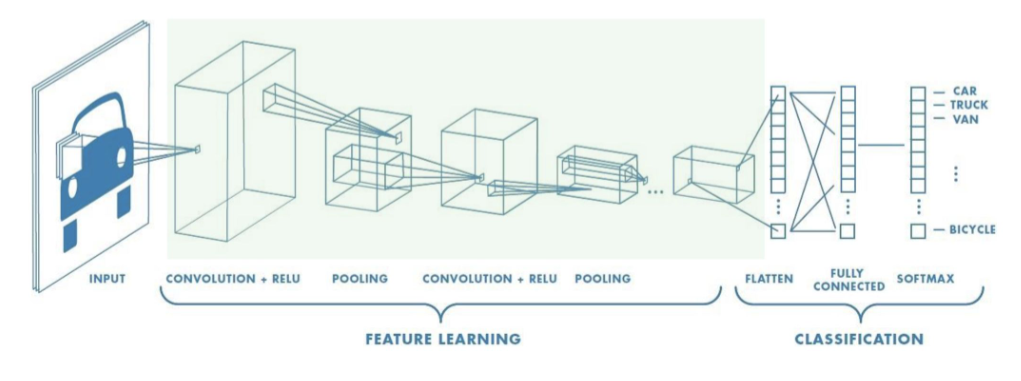
\includegraphics[width=0.5\linewidth]{endtoend.png}
    \caption{End-to-end network}
    \label{fig:enter-label}
\end{figure}

Thus, in a model that uses both fully connected and convolutional layers, the \textbf{CNN part is the encoder} and the \textbf{FC part is the classifier}. The CNN part extracts features, which are passed to the FC part that classifies the input. \\

\begin{idea}
    Because everything is \textbf{jointly connected, the weights} of the convolutional and fully connected layers are \textbf{jointly optimized} according to the loss function. This means that the \textbf{end-to-end} network is not going to face the same problem as the multi-stage algorithm described earlier.
\end{idea}

\textbf{The numbers in the kernel are learned through gradient descent.} \\

\textbf{Forward and Backward Pass (kernels):}
\begin{itemize}
    \item Initialize the kernels randomly
    \item In forward pass, convolve the image with the kernel
    \item In backward pass, update the kernel using gradients
\end{itemize}

\begin{figure}[h!t]
    \centering
    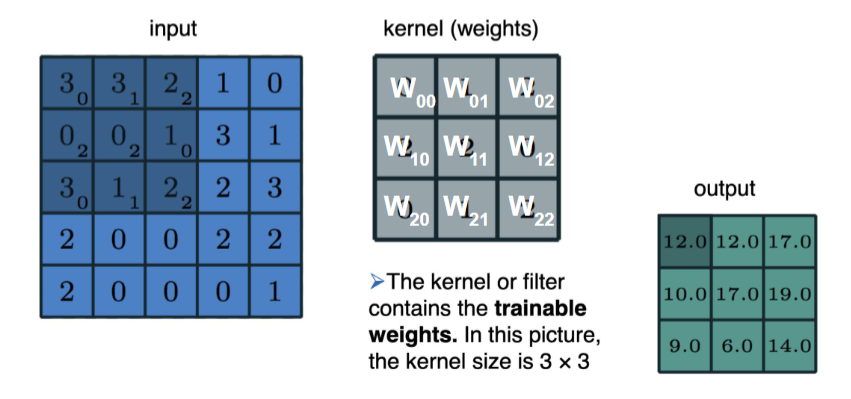
\includegraphics[width=0.5\linewidth]{forwardbackwardpass.png}
    \caption{Kernel as a matrix of weights}
    \label{fig:enter-label}
\end{figure}
\textbf{General CNN Terminology:}

\begin{definition}
    \textbf{Zero Padding:} adding zeros around the border of the image before convolution.
\end{definition}

\begin{figure}[h!t]
    \centering
    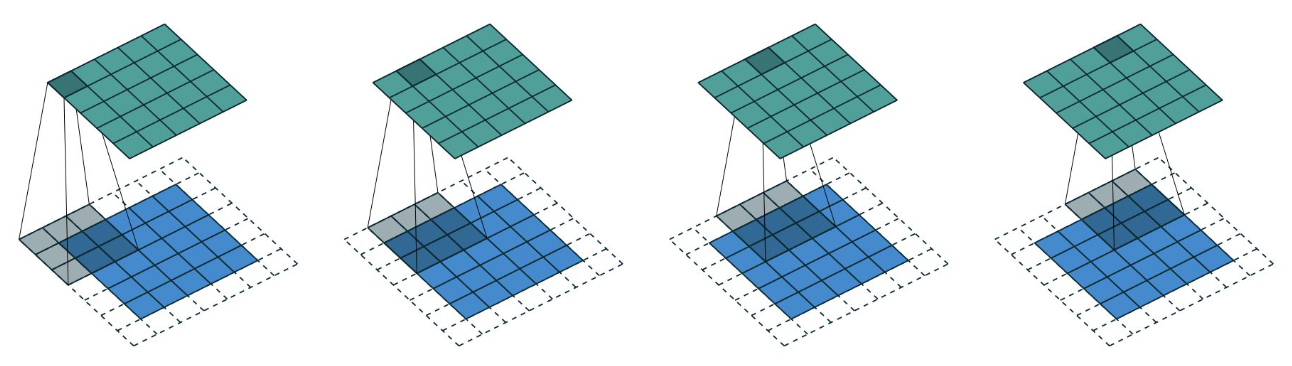
\includegraphics[width=0.75\linewidth]{zeropadding.png}
    \caption{Zero Padding}
    \label{fig:enter-label}
\end{figure}

\textbf{Zero padding is applied for two main reasons:}
\begin{enumerate}
    \item Keep width and height consistent with the previous layer
    \item Keep the information around the border of the image
\end{enumerate}

\begin{definition}
    \textbf{Stride:}  distance between two consecutive positions of the kernel.
\end{definition}

\begin{figure}[h!t]
    \centering
    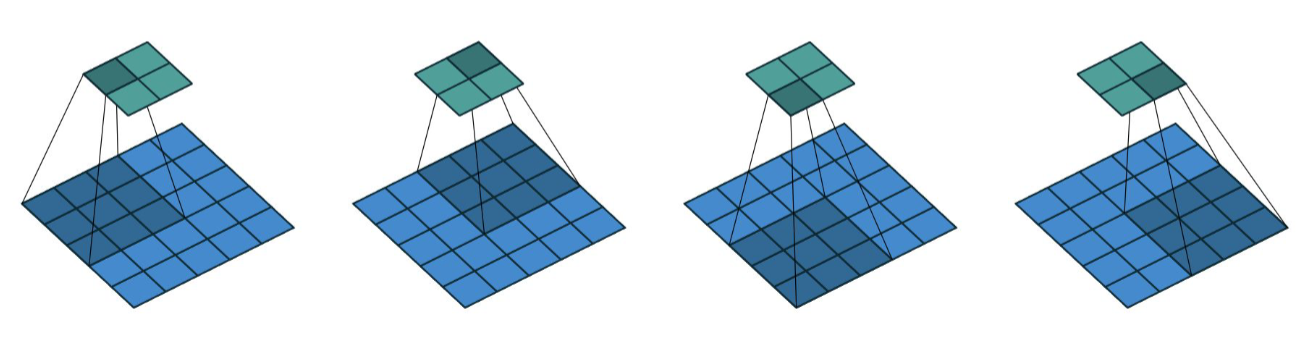
\includegraphics[width=0.75\linewidth]{stride.png}
    \caption{Stride}
    \label{fig:enter-label}
\end{figure}

Stride allows us to control the \textbf{output resolution}.

\begin{definition}
    \textbf{Feature Map:} a 2D or 3D array of values that represents the activations of specific features detected within an input data volume, generated by applying filters through convolutional operations in neural networks, particularly in convolutional neural networks (CNNs).
\end{definition}

\begin{theorem}
    \textbf{Computing the output size of the feature map (from convolving an image with a kernel)}\\

For each dimension of an input image with:
\begin{itemize}
    \item Image dimension of size \textbf{i}
    \item Kernel of size \textbf{k}
    \item Padding of size \textbf{p}
    \item Stride of size \textbf{s}
\end{itemize}
The size of output dimension is computed by:


\[o = [\frac{i + 2p - k}{s}] + 1\]
\\This equation assumes the kernel and image sizes are square!\\

\textbf{In the case that the sizes are not square}: 
    \begin{itemize}
        \item Image dimension of size \textbf{i x j}
        \item Kernel of size \textbf{k x l}
        \item Padding of size \textbf{p}
        \item Stride of size \textbf{s}
    \end{itemize}

We need to calculate the output of each dimension separately:

\[o_1 = [\frac{i + 2p - k}{s}] + 1\]
\[o_2 = [\frac{j + 2p - l}{s}] + 1\]
\end{theorem}

\begin{figure}[h!t]
    \centering
    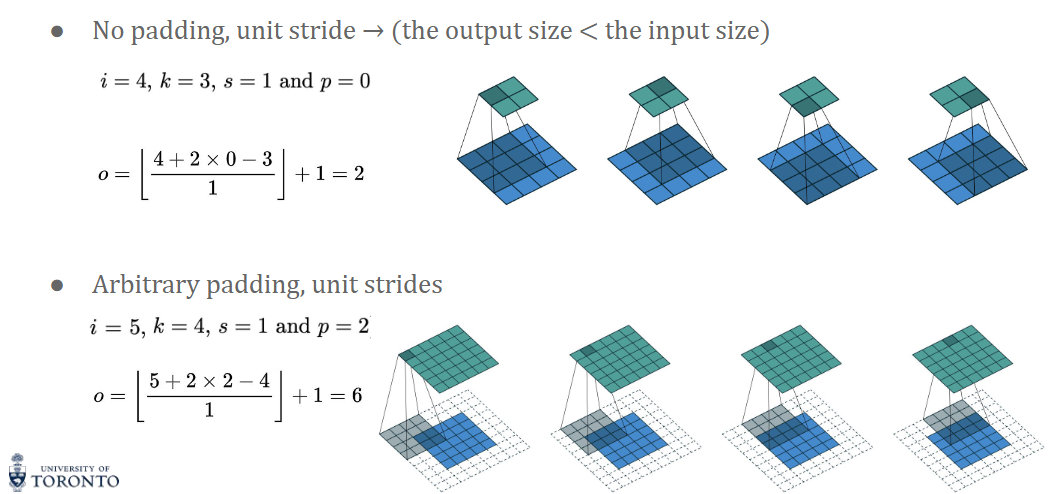
\includegraphics[width=0.8\linewidth]{convout1.png}
    \caption{Output Calculation Example 1}
    \label{fig:enter-label}
\end{figure}

\begin{figure}[h!t]
    \centering
    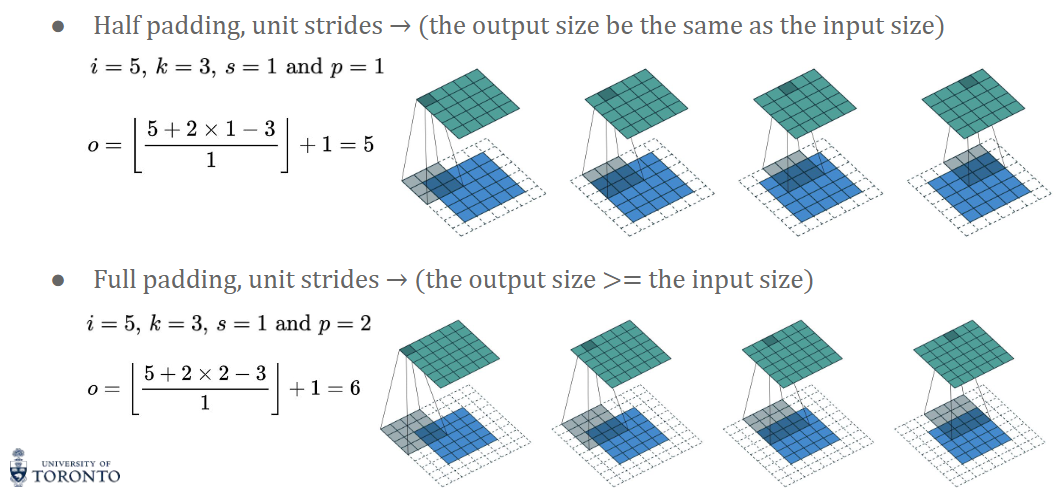
\includegraphics[width=0.8\linewidth]{outconv2.png}
    \caption{Output Calculation Example 2}
    \label{fig:enter-label}
\end{figure}

\begin{figure}[h!t]
    \centering
    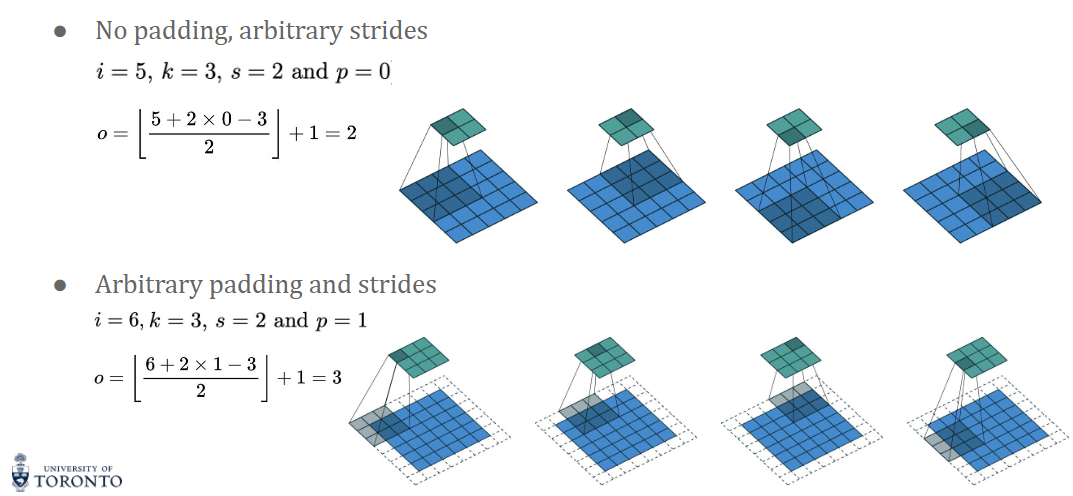
\includegraphics[width=0.8\linewidth]{outconv3.png}
        \caption{Output Calculation Example 3}
    \label{fig:enter-label}
\end{figure}

\newpage

\section{Convolution in 3D for RGB input}

In 3D, the kernel becomes a \textbf{3D tensor.}

\begin{figure}[h!t]
    \centering
    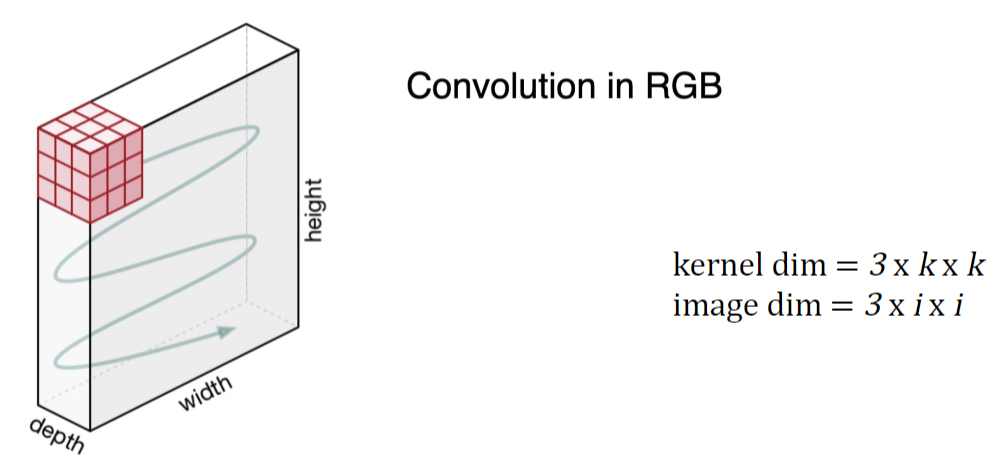
\includegraphics[width=0.5\linewidth]{conv3D.png}
    \caption{Convolution in 3D (RGB)}
    \label{fig:enter-label}
\end{figure}

\begin{example}
    \textbf{Calculating the number of trainable weights from an RGB input image and a convolution kernel}

    \begin{itemize}
        \item Colored input image: 3×28×28
        \item Convolution kernel: 3×3×3
    \end{itemize}

    The dimension of the kernel is 3 x 3 x 3, therefore there are \(3 x 3 x 3 = 27\) trainable weights.

\end{example}

\noindent\textbf{Expanding Feature Maps}

If we just use \textbf{one convolution, or one kernel, we are only able to detect one type of feature}, which isn't enough for information-rich images. The solution is to apply \textbf{multiple kernels at the same time to the image in parallel}, which will each extract a different feature, allowing for more than one feature to be extracted at a time. \\

\noindent Each kernel will produce an output, and these outputs will be stacked on top of each other to form the depths of the output.

\begin{figure}[h!t]
    \centering
    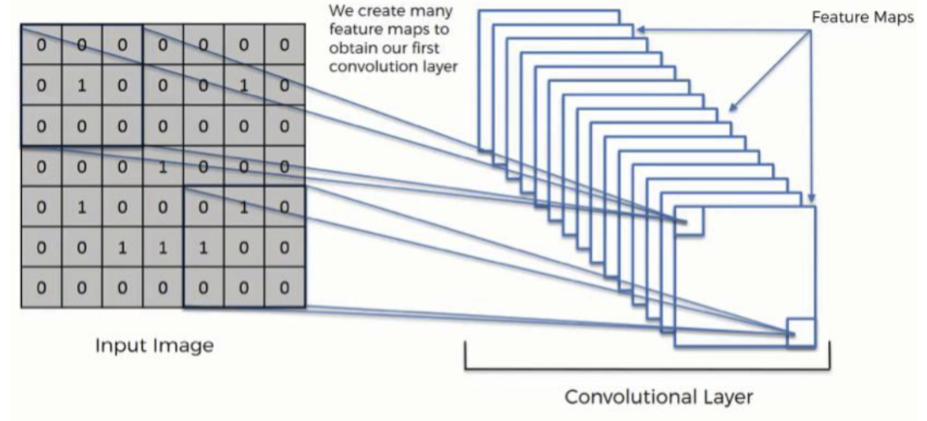
\includegraphics[width=0.5\linewidth]{expandingfeaturemaps.png}
    \caption{Applying multiple kernels}
    \label{fig:enter-label}
\end{figure}

\begin{theorem}
    The depths of the output = Number of kernels
\end{theorem}

\begin{figure}[h!t]
    \centering
    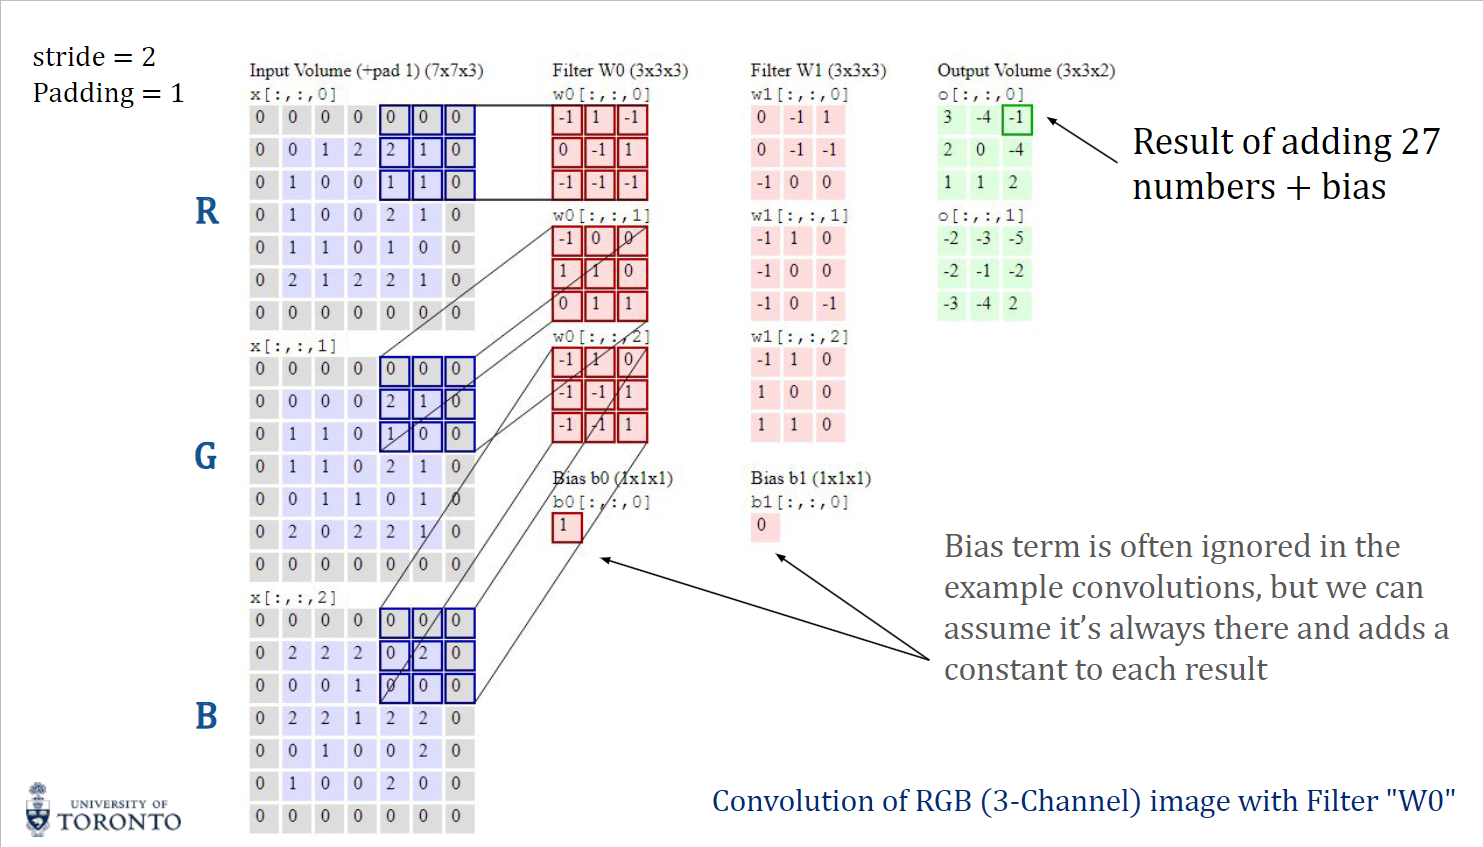
\includegraphics[width=0.75\linewidth]{examplemultiplekernels.png}
    \caption{Applying multiple kernels}
    \label{fig:enter-label}
\end{figure}

\begin{example}
    \textbf{Calculating the number of input channels, output channels, and trainable weights from an RGB input image and a convolution kernel}

    \begin{itemize}
        \item \textbf{Colored input image: 3×28×28}
        \item \textbf{Convolution kernel: 5x3×8×8 }
        \begin{itemize}
            \item There are 5 kernels being applied in parallel. There are each 3x8x8 in size
        \end{itemize}
    \end{itemize}

\begin{itemize}
    \item Input channels: 3 input channels because the depth of the input image is 3
    \item Output channels: 5 output channels because there are 5 kernels
    \item  Trainable weights: 5 x 3 x 8 x 8 = 960 (weights) + 5 (bias for each kernel)
\end{itemize}

\end{example}

\textbf{What is preventing these filters from learning the same features?}
\begin{itemize}
    \item \textbf{Random Initialization}: we assign random initial weights to the kernels which cause them to all learn different features
\end{itemize}


\section{Pooling Operator}
In order to \textbf{consolidate information and remove information that is not useful} with convolutional layers, we can use pooling operators or strided convolutions. Compressing information allows the network to establish the most \textbf{foundational features or "elements" of a class} so that it may \textbf{generalize well to unseen data.} As we go deeper into the network, we compress the data more and more.

\begin{definition}
    \textbf{Pooling Operator:} a \textbf{downsampling} technique that reduces the spatial dimensions of the input data by aggregating information from neighboring elements. It aims to capture important features while decreasing the computational complexity and memory requirements of the network. 
\end{definition}

\textbf{Max Pooling}

\begin{itemize}
    \item pooling layers provide \textbf{invariance to small translations} of the input
\end{itemize}
\begin{figure}[h!t]
    \centering
    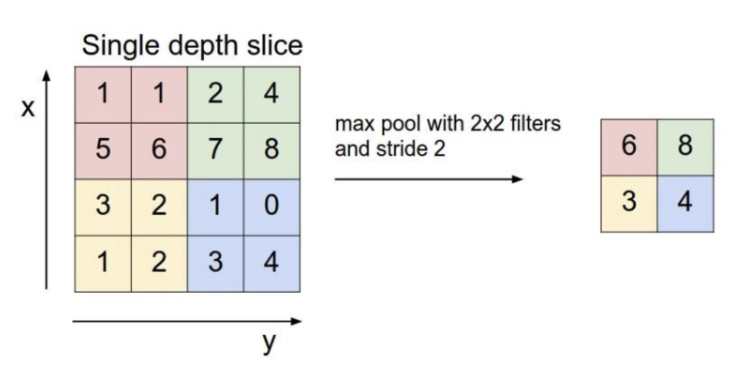
\includegraphics[width=0.5\linewidth]{maxpooling.png}
    \caption{Max Pooling}
    \label{fig:enter-label}
\end{figure}

\begin{definition}
    \textbf{Max Pooling:} a pooling operator used to downsample the spatial dimensions of input data. It involves \textbf{dividing the input into non-overlapping regions and selecting the maximum value from each region}, effectively capturing the most prominent feature within that region.
\end{definition}

\begin{theorem}
    The size of max pooling output is computed by:

\[o = [\frac{i - k}{s}] + 1\]
Where:
\begin{itemize}
    \item Image dimension of size \( i \)
    \item  Kernel of size \( k \)
    \item Stride of size \(s\)
\end{itemize}
\end{theorem}

\textbf{Average Pooling}
\begin{itemize}
    \item usually \textbf{less effective} than max pooling
\end{itemize}
\begin{figure}[h!t]
    \centering
    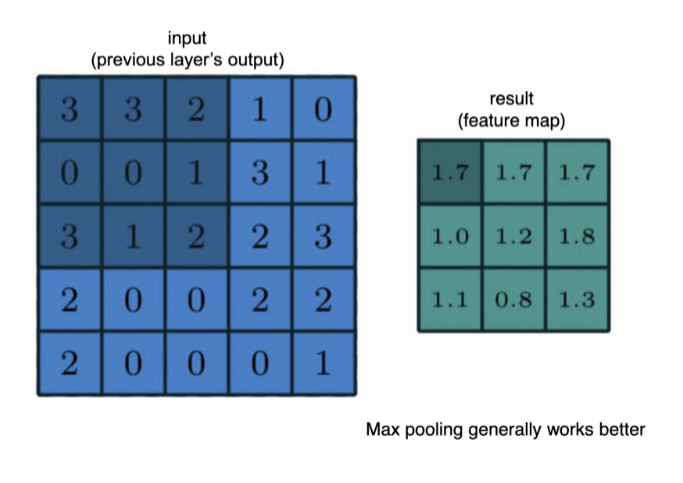
\includegraphics[width=0.4\linewidth]{averagepooling.png}
    \caption{Average Pooling}
    \label{fig:enter-label}
\end{figure}
\begin{definition}
    \textbf{Average Pooling:}  a pooling operator used to downsample the spatial dimensions of input data. It involves \textbf{dividing the input into non-overlapping regions and calculating the average value} of the elements within each region. 
\end{definition}

\textbf{Strided Convolutions}
\begin{itemize}
    \item More recently, people are doing away with pooling operations, using strided convolutions instead
    \item Shift the kernel by s (eg. s = 2) when computing convolution
\end{itemize}
\begin{figure}[h!t]
    \centering
    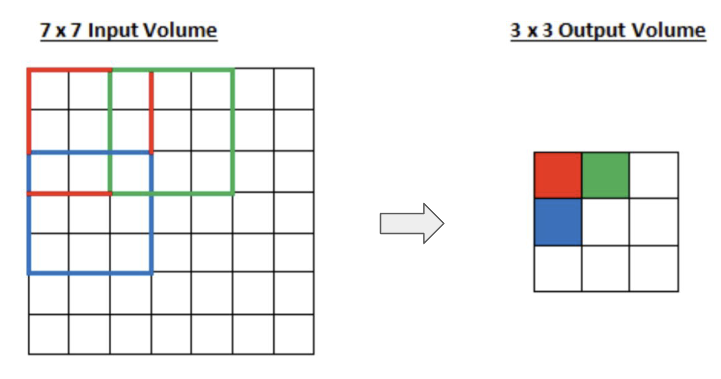
\includegraphics[width=0.45\linewidth]{stridedconvolution.png}
    \caption{Strided Convolutions}
    \label{fig:enter-label}
\end{figure}

\begin{definition}
    \textbf{Strided Convolutions:} a downsampling technique that combines convolution and pooling. It involves \textbf{applying convolutional operations with larger strides} (spacing between filter placements) \textbf{than usual}, resulting in reduced spatial dimensions and aggregated feature representation. 
\end{definition}

\begin{idea}
    As we go through a CNN network layer by layer:
    \begin{itemize}
        \item The filter\textbf{ depth increases} (as the number of kernels increases)
        \begin{itemize}
            \item The kernels closer to the input learn low level features
            \begin{itemize}
                \item Due to the hierarchical nature of information, the number of kernels must increase to extract more detailed (high-level) features
                \item That being said, kernel size generally is fixed
            \end{itemize}
        \end{itemize}
        \item The feature map height and width decreases
    \end{itemize}
\end{idea}

\begin{figure}[h!t]
    \centering
    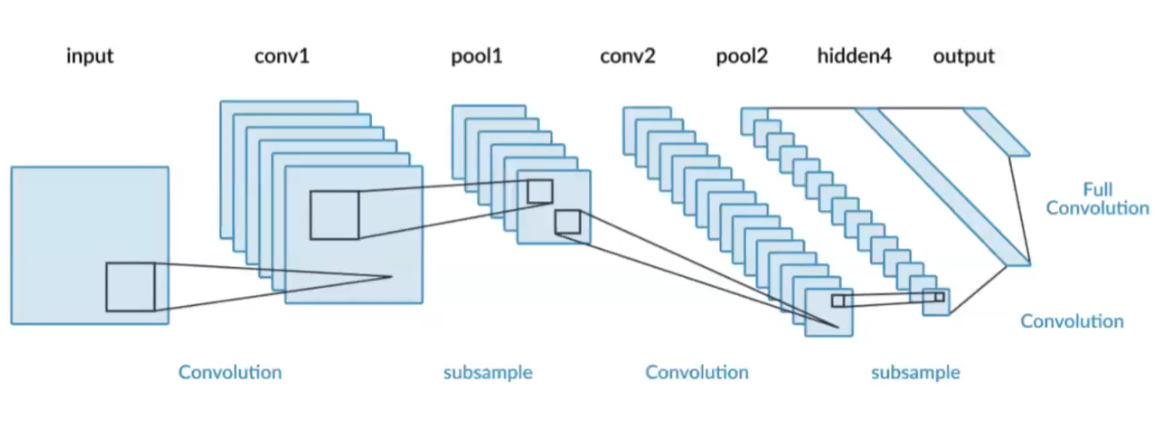
\includegraphics[width=0.75\linewidth]{cnn.png}
    \caption{CNN}
    \label{fig:enter-label}
\end{figure}

\section{PyTorch Implementation}

\begin{example}
  \textbf{  Syntax for defining a convolutional layer:}

\begin{verbatim}
    self.conv1 = nn.Conv2d(in_channels, out_channels, kernel_size, stride, padding)
\end{verbatim}
in\_channels and out\_channels are int. kernel\_size, stride, padding may be either int tuple. By default, stride is 1 and padding is 0.

\end{example}

\begin{example}
    \textbf{Syntax for defining a pooling layer:}\\

Max Pool:
\begin{verbatim}
    self.pool = nn.MaxPool2d(kernel_size, stride)
\end{verbatim}
Average Pool:
\begin{verbatim}
    self.pool = nn.AvgPool2d(kernel_size, stride)
\end{verbatim}
\end{example}

\begin{figure}[h!t]
    \centering
    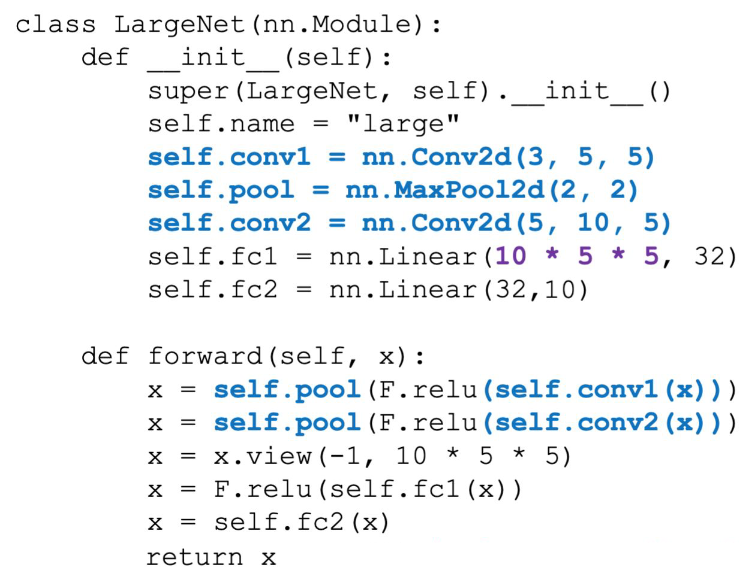
\includegraphics[width=0.5\linewidth]{samplecnnpytorch.png}
    \caption{Example CNN in PyTorch}
    \label{fig:enter-label}
\end{figure}


\section{Visualizing Convolutional Filters}

\textbf{What do CNN Filters/Feature maps look like?}

\begin{figure}[h!t]
    \centering
    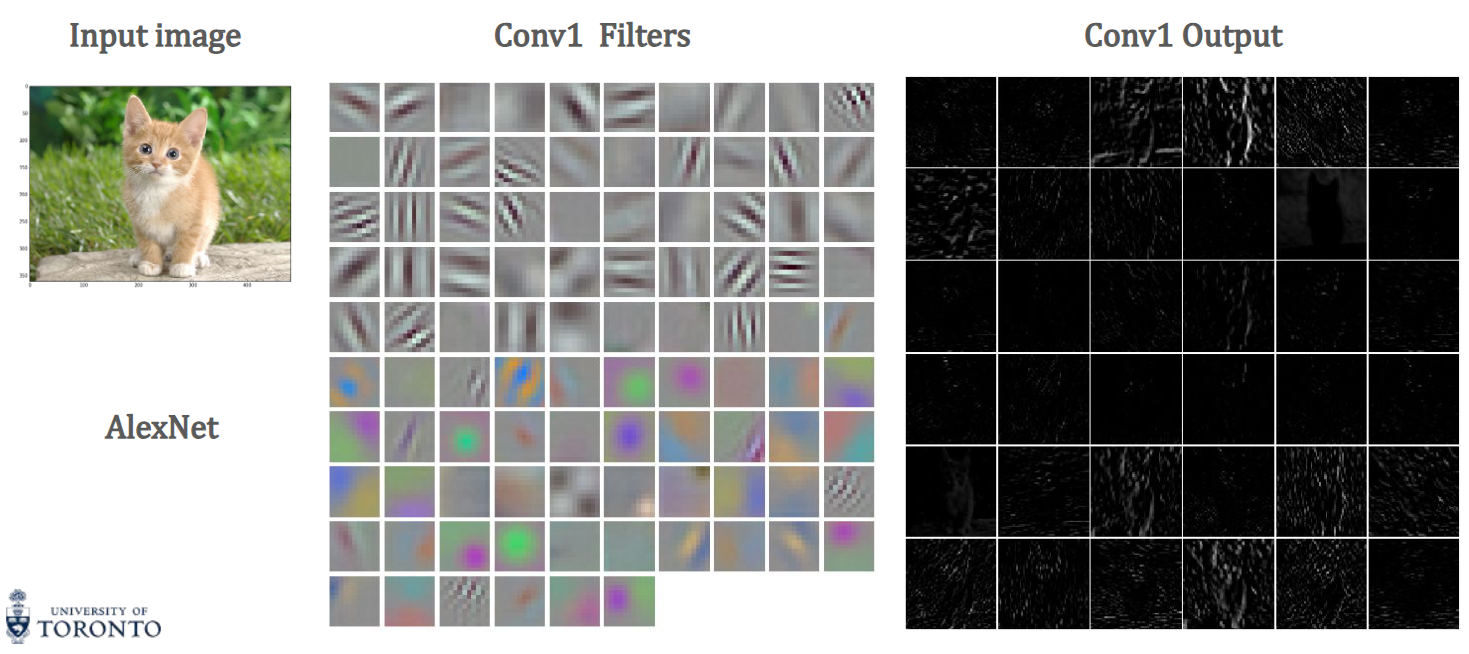
\includegraphics[width=0.4\linewidth]{cnnfilters.png}
    \caption{Example of a CNN filter}
    \label{fig:enter-label}
\end{figure}

\textbf{What features do CNNs learn?}

\begin{figure}[h!t]
    \centering
    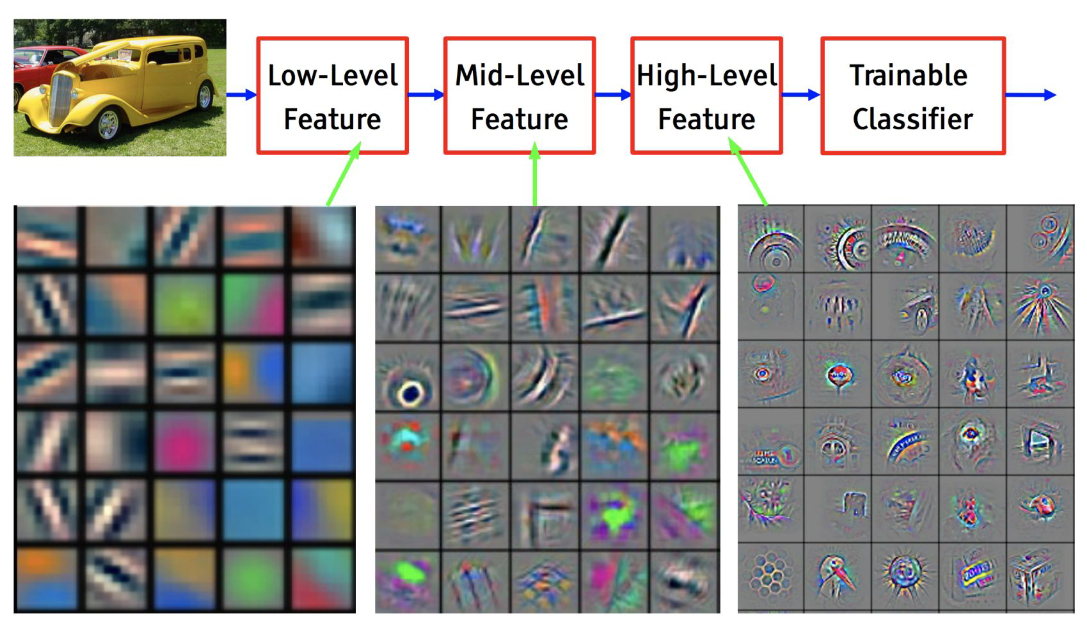
\includegraphics[width=0.5\linewidth]{learnedfeaturescnn.png}
    \caption{Learned Features}
    \label{fig:enter-label}
\end{figure}


\begin{definition}
    \textbf{Saliency Maps:} are visual representations highlighting the most important and relevant regions or features within an image, indicating where the human visual attention is likely to be drawn.
\end{definition}

\begin{figure}[h!t]
    \centering
    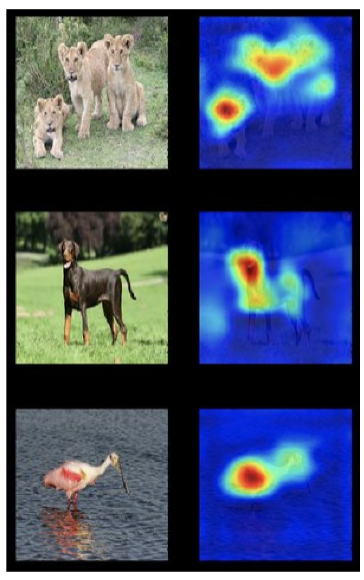
\includegraphics[width=0.25\linewidth]{saliencymap.png}
    \caption{Saliency Maps}
    \label{fig:enter-label}
\end{figure}

\begin{enumerate}
    \item Feed the image to the network
    \item Compute the gradients back to the input image
    \item Take the maximum value of absolute gradients across channels
    \item Visualize
\end{enumerate}

\begin{itemize}
    \item Saliency maps use gradients of the output over the input to highlight the areas of the images which are relevant for the classification
    \item Unfortunately outside giving some intuition, these are not practically very useful, and sometimes even misleading
    \item However, they can be used as a debugging tool to check if model is looking at the right features
\end{itemize}
\newpage

\section{Pre-Deep Learning Era}

\textbf{LeNet}

\begin{itemize}
    \item Convolutional Neural Networks were first introduced by Yann LeCun in 1989
    \begin{itemize}
        \item Based on earlier "Neocognitron", but little used model (Fukushima, 1980)
    \end{itemize}
    \item Several variants, mostly we refer to LeNet-5 (above, 1998)
    \begin{itemize}
        \item 7 layers total, 2 convolutional, 2 pooling, 3 fully-connected
    \end{itemize}
\end{itemize}

\begin{figure}[h!t]
    \centering
    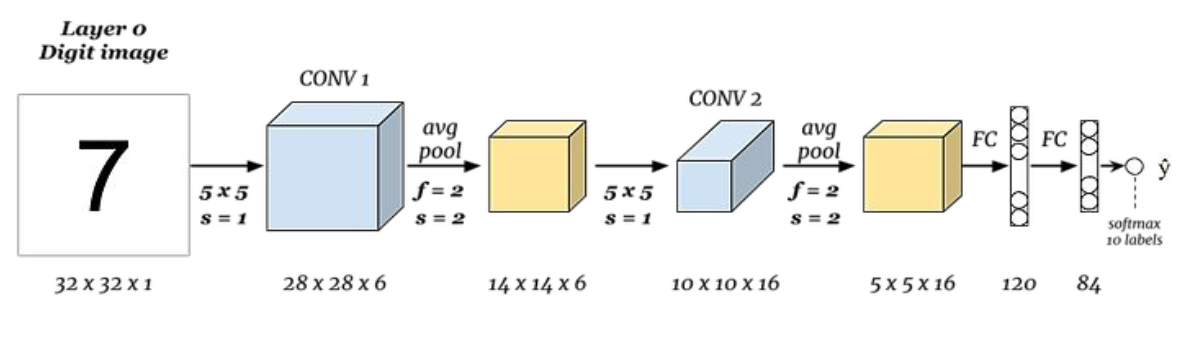
\includegraphics[width=1\linewidth]{lenet.png}
    \caption{LeNet CNN}
    \label{fig:enter-label}
\end{figure}

\begin{itemize}
    \item Due to heavy hardware constraints at the time, training this network was a pain in the ass. However, once it was working, several useful properties were observed:
\end{itemize}

\begin{figure}[h!t]
    \centering
    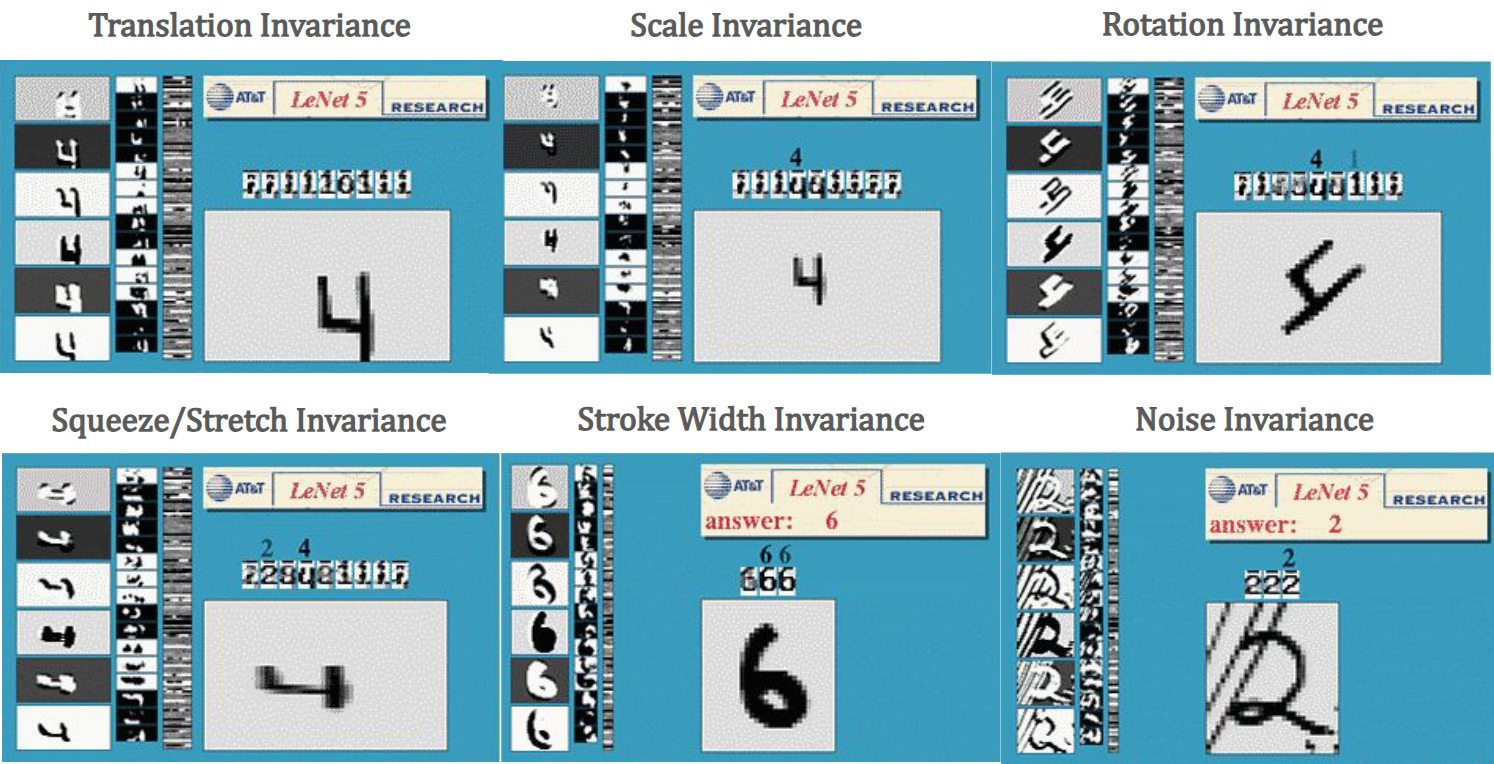
\includegraphics[width=0.8\linewidth]{lenetletters.png}
    \caption{LeNet Properties}
    \label{fig:enter-label}
\end{figure}

With PyTorch, implementation of this model is simple. 

\begin{figure}[h!t]
    \centering
    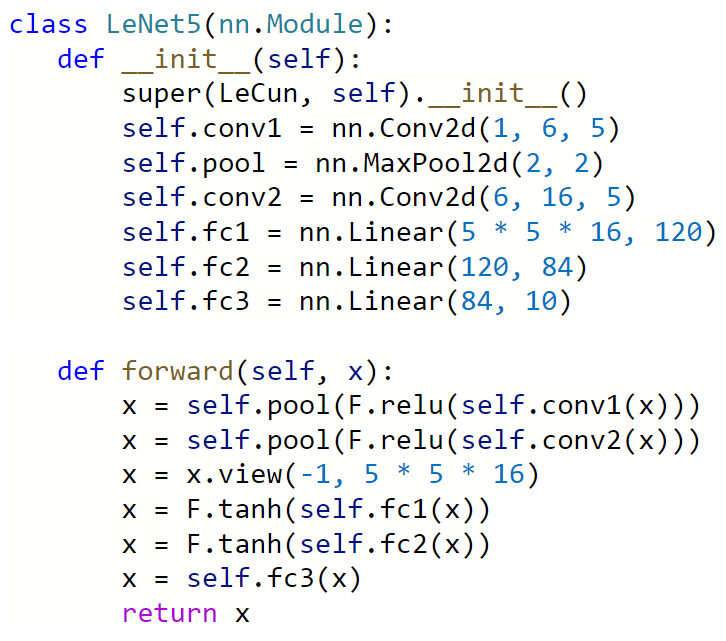
\includegraphics[width=0.5\linewidth]{lenetpy.png}
    \caption{PyTorch Implementation of LeNet}
    \label{fig:enter-label}
\end{figure}

\newpage

\textbf{On the Eve of Deep Learning:}
\begin{itemize}
    \item We took a break in the mid-90s! ... let's skip forward to 2010
    \item Visual Object Classification is holy grail of Computer Vision
    \begin{itemize}
        \item Classification of object is in an image, e.g. dog v.s. cat
    \end{itemize}
    \item Best solutions to Object Classification is based on \textbf{Deformable Parts Models}
    \item CNNs Are outperformed on most tasks by using hand-crafted computer vision features (algorithms), and other ML classifiers, e.g. random forests (decision trees) or SVM
\end{itemize}

An intuitive way of recognizing a face is searching for facial features in an image. The problem with this idea is that if we look for face parts, we will identify a face even if the face parts are in the wrong locations.

\begin{figure}[h!t]
    \centering
    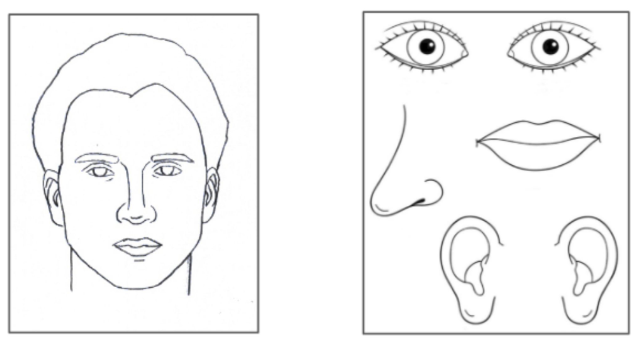
\includegraphics[width=0.35\linewidth]{deformablepartsmodel.png}
    \caption{Looking for facial features alone isn't good enough}
    \label{fig:enter-label}
\end{figure}

\textbf{Deformable Parts Models}

\begin{definition}
    \textbf{Deformable Parts Models:} a class of object detection models in computer vision that incorporate flexible part structures within an object to improve accuracy in recognizing complex objects with varying appearances and poses.
\end{definition}

\begin{itemize}
    \item Recognize using parts and locations of parts
    \item Allow some deformation of part location, as there are difference in facial structure among different populations
    \item However, this is hard to extend to many different types of objects!
    \item Also doesn't work well for different viewing angles
\end{itemize}

\begin{figure}[h!t]
    \centering
    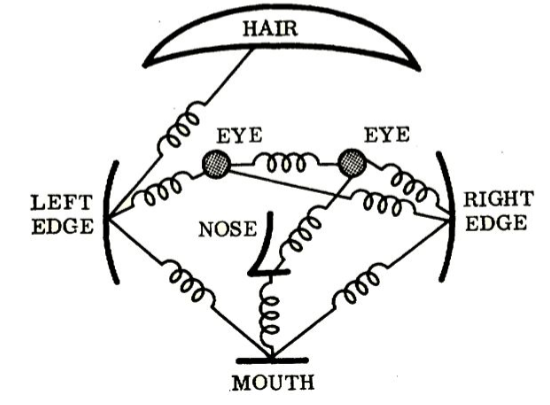
\includegraphics[width=0.35\linewidth]{dpm.png}
    \caption{Deformable Parts Models}
    \label{fig:enter-label}
\end{figure}

\begin{idea}
    Intuition as to how CNNs work is based on Deformable Parts Models
\end{idea}

\section{Modern Architectures}

\textbf{ImageNet Large Scale Visual Recognition Challenge}

\begin{definition}
   \textbf{ImageNet Large Scale Visual Recognition Challenge (ILSVRC):} is an annual competition in computer vision where participants develop and train machine learning models to classify and detect objects within a large dataset of images, known as ImageNet, containing thousands of categories.
\end{definition}

\begin{itemize}
    \item Pascal VOC was around 20,000 images with 20 classes (2006 - 2009)
    \begin{itemize}
        \item Around the 2010s, this was the largest dataset available
    \end{itemize}
    \item ImageNet was the first large-scale image dataset (14 million images)
    \item ILSVRC dataset based on ImageNet
    \begin{itemize}
        \item 1 Million training images
    \end{itemize}
    \begin{itemize}
        \item 1000 different classes!
    \end{itemize}
    \begin{itemize}
        \item 50k validation, test set (never released)
    \end{itemize}
    \item When we say ImageNet, we mean ILSVRC
\end{itemize}

\begin{figure}[h!t]
    \centering
    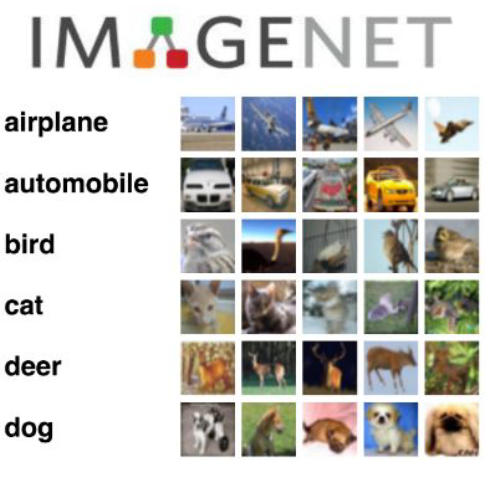
\includegraphics[width=0.225\linewidth]{imagenet.png}
    \caption{Image Net}
    \label{fig:enter-label}
\end{figure}

\begin{itemize}
    \item ILSVRC challenge ran from 2010.
    \item Like Pascal VOC, every year saw the new winner improve accuracy by ~1-2\%
    \item CNN entry (AlexNet) in 2012 improved accuracy over previous year by ~10\%
    \item This is when "Deep Learning" began
\end{itemize}

\textbf{AlexNet}

\begin{figure}[h!t]
    \centering
    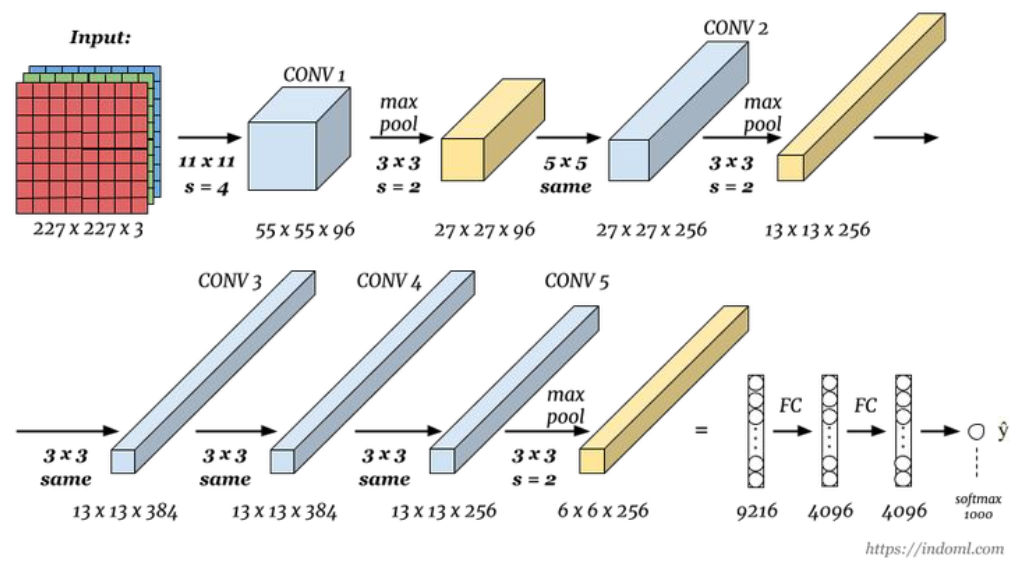
\includegraphics[width=0.75\linewidth]{alexnet.png}
    \caption{AlexNet Architecture}
    \label{fig:enter-label}
\end{figure}

\noindent \textbf{Deep Learning is differentiated from vanilla Neural Networks mostly in the changes between LeNet-5 and AlexNet:}
\begin{itemize}
  \item Much larger training datasets (e.g. ImageNet)
  \item Vast increase in compute/GPU acceleration (imagine 1989 PC v.s. 2012!)
  \item Much larger model size/more layers, enabled by both of the above!
\end{itemize}
\textbf{AlexNet Training/Architecture Improvements:}
\begin{itemize}
  \item Large number of convolutional layers (i.e. deeper model)
  \item Use ReLU activation functions instead of sigmoids
  \item Dropout, data augmentation
\end{itemize}
\textbf{About AlexNet Training:}
\begin{itemize}
  \item $\sim$60 Million parameters!
  \item Used GPUs to accelerate compute: 2 Nvidia GTX 580 GPUs
  \item 5-6 days to train over 90 epochs
  \item Optimized with SGD + Momentum
  \item Uses weight decay, dropout \& data augmentation to improve generalization
  \item Learning rate schedule decreased learning rate 3 times over training
\end{itemize}

\noindent\textbf{Data Augmentation}

\begin{definition}
    \textbf{Data Augmentation:} refers to the technique of artificially increasing the diversity of a dataset used for training machine learning models by applying various transformations, modifications, or perturbations to the original data, resulting in augmented samples that enhance the model's ability to generalize and perform better on unseen data.
\end{definition}
\begin{itemize}
    \item Apply class-preserving transformations to the input
    \item Increases training data
    \item Helps generalization by learning internal representation of transformations
    \begin{itemize}
        \item Helps the model learn the appearance in different situations (eg. low lighting, different weather conditions)
    \end{itemize}
    \item Used by AlexNet (and all other CNNs)

\end{itemize}

\begin{figure}
    \centering
    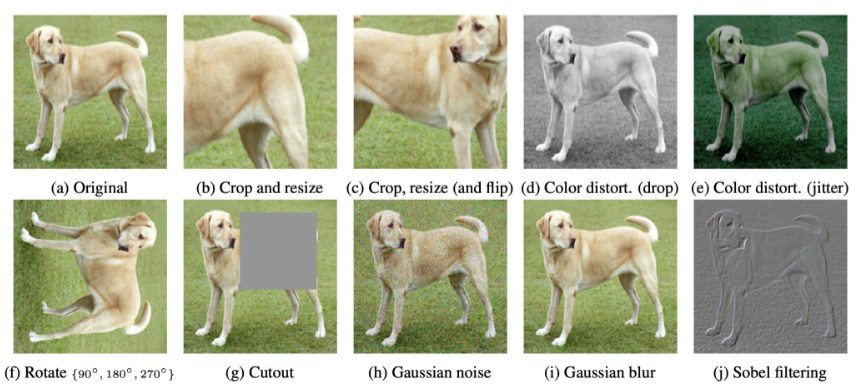
\includegraphics[width=0.75\linewidth]{dataaugmentation.png}
    \caption{Ways to apply Data Augmentation}
    \label{fig:enter-label}
\end{figure}

\noindent\textbf{Generalization and Depth}\\

AlexNet and following models showed that increased depth improved generalization on ILSVRC, and other tasks. However, training very deep models often failed! This was due to \textbf{vanishing or exploding gradients}. The most important improvements in the past 10 years have been to address this:
\begin{itemize}
  \item Improved initialization for ReLUs
  \item Normalization (e.g. Batch Normalization)
  \item Residual connections
\end{itemize}

\noindent\textbf{GoogleLeNet (Inception)}\\

People were catching on to the idea that \textbf{increased depth improved generalization}. This was the main motivation behind GoogleLeNet.

\begin{itemize}
    \item 2014 ILSVRC winner, 6.67\% Top-5 error
    \begin{itemize}
        \item Human gets ~5.1\%
    \end{itemize}
    \item Primary motivation was to go deeper
    \begin{itemize}
        \item 22 convolutional layers
    \end{itemize}
    \item Much more parameter efficient than AlexNet
    \begin{itemize}
        \item 4 million vs. 60 million for AlexNet
    \end{itemize}
\end{itemize}

Rather than trying to figure out the optimal kernel size for each layer, they said, "why not \textbf{use all of them at the same time}?"

\begin{itemize}
    \item The inception block uses a mixture of 3x3, 5x5 and 7x7 filters on one layer
    \item We don't need large 7x7 (or 11x11 as in AlexNet) to learn most important filters.
    \item We can use mostly 3x3, and add a few larger filters
\end{itemize}

\begin{figure}[h!t]
    \centering
    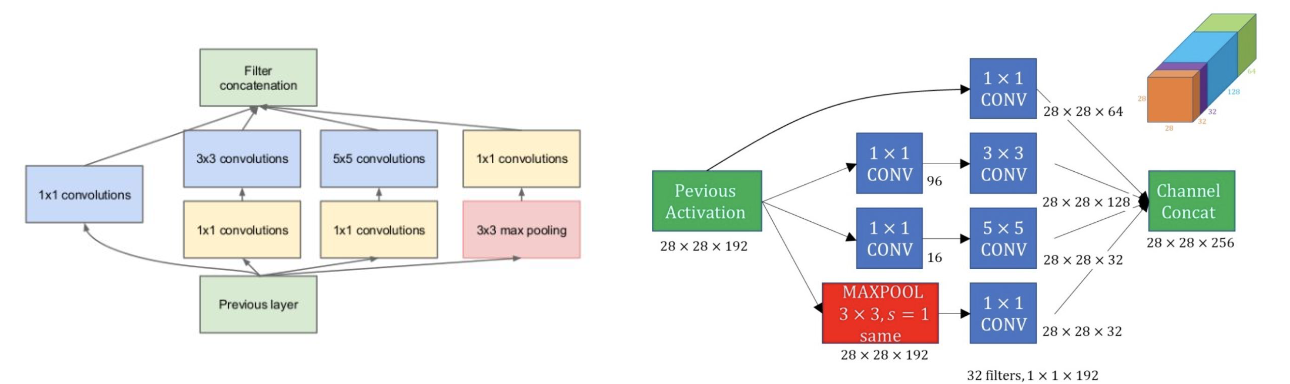
\includegraphics[width=0.75\linewidth]{inceptionblock.png}
    \caption{Ensemble Learning}
    \label{fig:enter-label}
\end{figure}

Interestingly, they used 1 x 1 convolution, which means each kernel is applied to one pixel.\\

\textbf{Pointwise (1x1) Convolution}
\begin{itemize}
    \item \textbf{Pixel-wise linear transformations!}
    \begin{itemize}
        \item Originally used in a model called "Network-in-Network"
    \end{itemize}
    \begin{itemize}
        \item With a non-linearity, they are non-linear pixel-wise transformations
    \end{itemize}
    \item Learn to map CNN feature maps into a lower or higher dimensional space
    \begin{itemize}
        \item Good for learning compact representations/compression
    \end{itemize}
    \item Efficiently \textbf{control the depths} of the network in different layers \textbf{while maintaining resolution}
    \item Used in all modern CNN architectures (except VGG)

\end{itemize}

\begin{figure}[h!t]
    \centering
    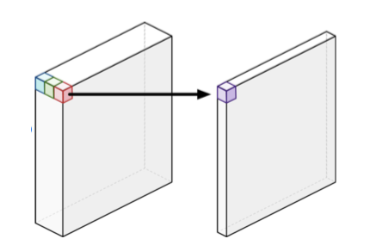
\includegraphics[width=0.35\linewidth]{pointwiseconvolution.png}
    \caption{Pointwise Convolution}
    \label{fig:enter-label}
\end{figure}

Using pointwise convolution, they managed to reduce the number of parameters to a relatively small number.\\

\textbf{Auxiliary Loss}

\begin{definition}
    \textbf{Auxiliary Loss:} refers to an \textbf{additional loss function} incorporated into a model's training process alongside the main objective. It aims to provide auxiliary supervision to intermediate layers, helping the network learn relevant features and improve convergence.
\end{definition}

\begin{figure}[h!t]
    \centering
    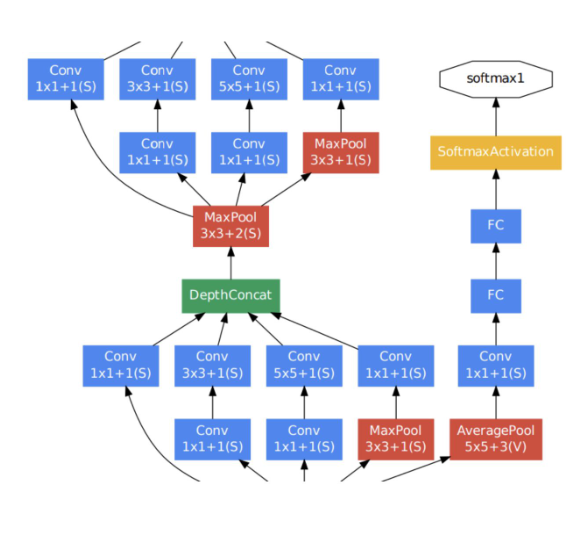
\includegraphics[width=0.4\linewidth]{auxiliaryloss.png}
    \caption{Auxiliary Loss}
    \label{fig:enter-label}
\end{figure}

\begin{itemize}
    \item \textbf{Inception network is pretty deep} → subject to the vanishing gradient problem.
    \item \textbf{Solution} → intermediate classifiers
    \item Adding classifiers in the intermediate layers such that the final loss is a combination of the intermediate losses and the final loss.
\end{itemize}

\textbf{VGG (Visual Geometry Group, Oxford)}

\begin{itemize}
    \item 2014 ILSVRC classification 2nd place, 7.3\% Top-5 error
    \begin{itemize}
        \item However, won parallel ILSVRC localization challenge
    \end{itemize}
    \item Proposed Models with 11, 13, 16, and 19 layers
    \item Very simple architecture, easy to understand/extend
    \item Very large number of parameters: 138 Million v.s. 60 Million for AlexNet!
\end{itemize}

\begin{figure}[h!t]
    \centering
    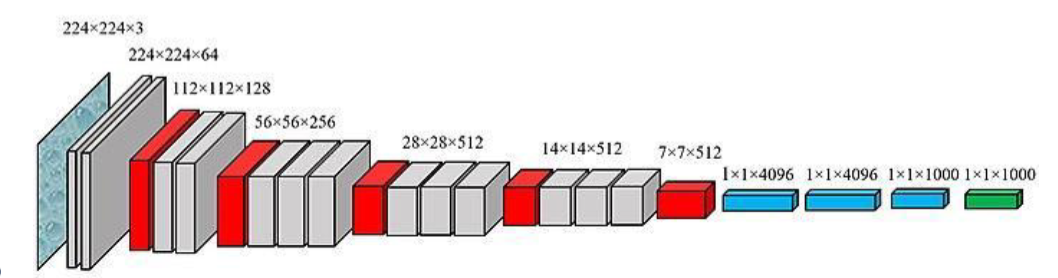
\includegraphics[width=0.75\linewidth]{vgg.png}
    \caption{Visual Geometry Group}
    \label{fig:enter-label}
\end{figure}

VGG was a very impactful paper:

\begin{itemize}
    \item Simple architecture made of simple stacked blocks
\item \textbf{We only need 3x3 filters} (set the modern standard)
\begin{itemize}
    \item Authors pointed out that stacked 3x3 filters can approximate any larger-sized convolution, more efficiently
    \item Since VGG almost all CNNs use mostly/exclusively 3x3 filters!
\item \textbf{The data augmentation used by VGG is very commonly used}
\end{itemize}

\end{itemize}

\begin{figure}[h!t]
    \centering
    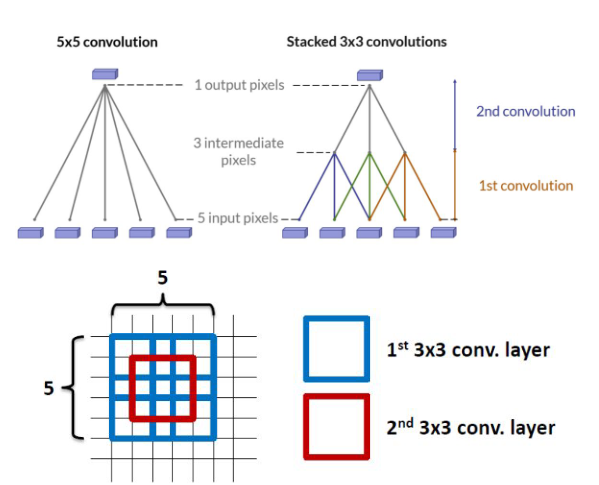
\includegraphics[width=0.5\linewidth]{vgg2.png}
    \caption{VGG's Simple Architecture}
    \label{fig:enter-label}
\end{figure}
\begin{figure}[h!t]
    \centering
    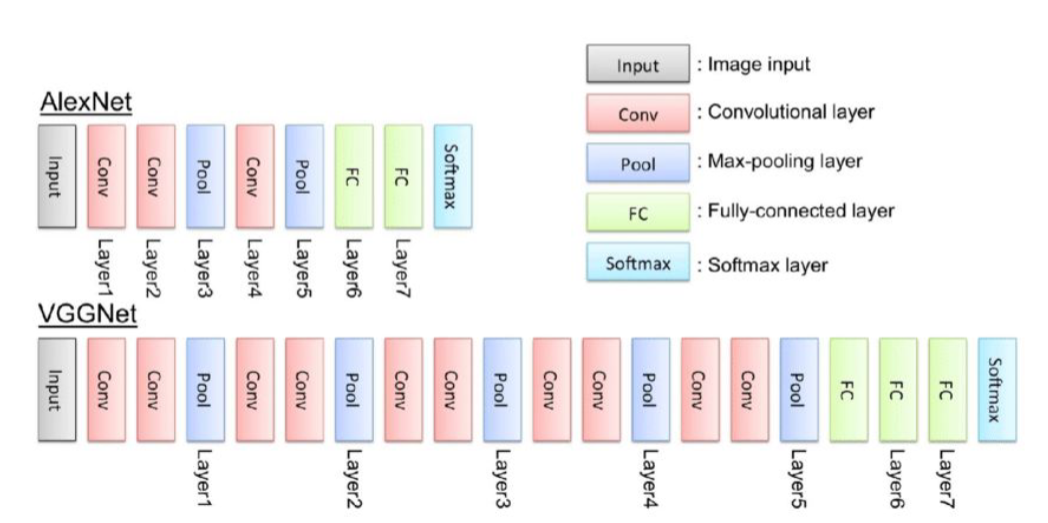
\includegraphics[width=0.5\linewidth]{vggvsalex.png}
    \caption{AlexNet vs. VGG}
    \label{fig:enter-label}
\end{figure}

\textbf{Residual Networks (ResNet)}\\

Even with Batch Normalization and ReLUs, training very deep networks fails. ResNet addresses this by using \textbf{skip connections (shortcuts)} to provide deeper layers with more direct access to signals that might otherwise be lost due to vanishing gradients. \\

\begin{figure}[h!t]
    \centering
    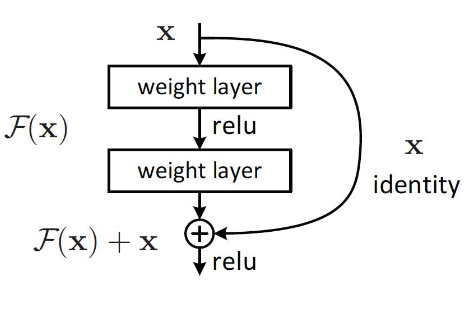
\includegraphics[width=0.35\linewidth]{resnet.png}
    \caption{ResNet Skip Connections}
    \label{fig:enter-label}
\end{figure}

ResNet won ILSVRC 2015 with a 3.57\% error rate.
\begin{itemize}
    \item Model had 152 layers,
    \item Better than the Human baseline!
\end{itemize}

\begin{definition}
    \textbf{Skip Connections:} a technique where the output of one layer or block of layers is combined with the output of a previous layer. This helps mitigate issues like vanishing gradients and aids in training deeper neural networks by allowing information to flow more directly across layers.
\end{definition}

\begin{figure}
    \centering
    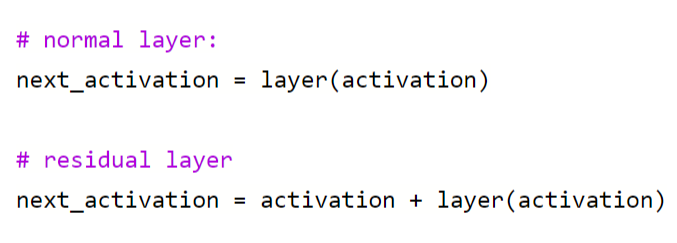
\includegraphics[width=0.5\linewidth]{resnetpy.png}
    \caption{PyTorch Implementation of Skip Connections}
    \label{fig:enter-label}
\end{figure}

\begin{figure}[h!t]
    \centering
    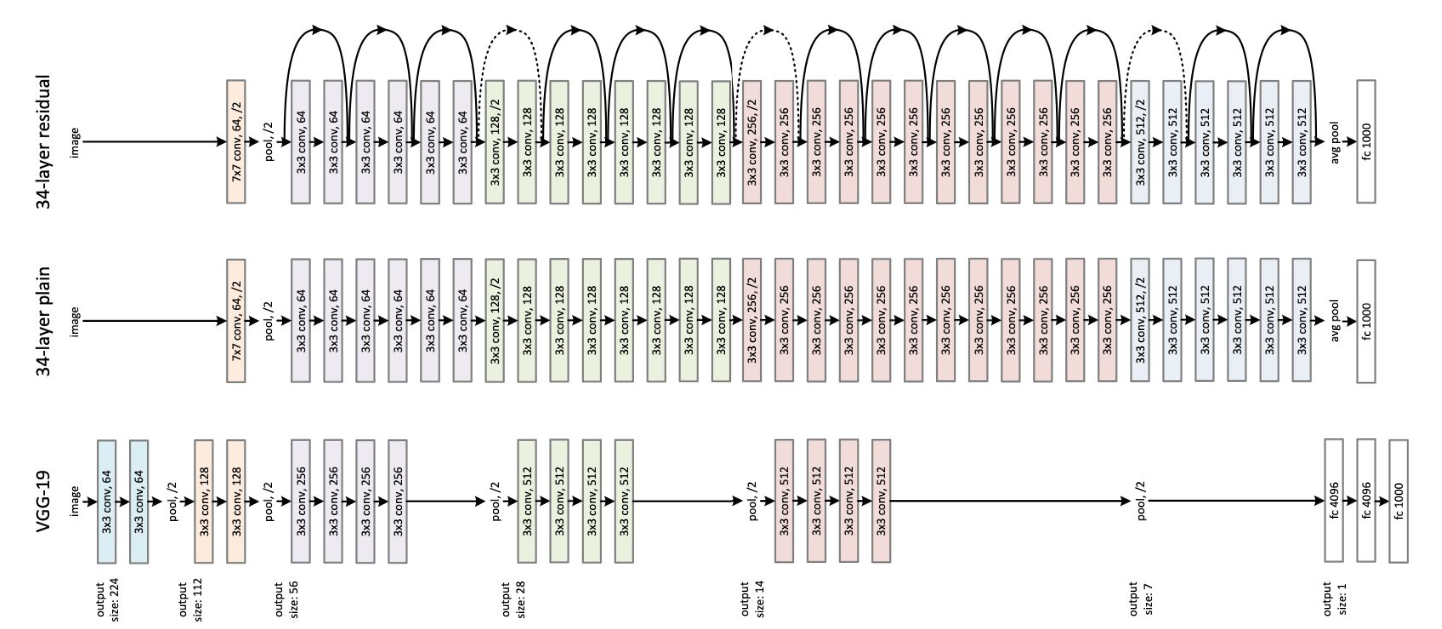
\includegraphics[width=1\linewidth]{resnetandothers.png}
    \caption{ResNet compared to others}
    \label{fig:enter-label}
\end{figure}

In this diagram, we notice the following:
\begin{itemize}
    \item \textbf{Residual blocks} (multiple convolutions with skip connections)
    \item \textbf{Downsampling using stride 2}, instead of max/avg pooling (strided convolution)
    \item \textbf{Global average pooling} after last convolutional layers (introduced by Network-in-Network)
    \begin{itemize}
        \item Means that the embedding has no spatial dimension and is only 512 floats!
    \end{itemize}
    \item Only \textbf{a single fully-connected classification layer}
    \begin{itemize}
        \item learned embeddings are so good we don't need a complex classifier at end of model
        \item allows variable input sizes because it's not constrained by FC layer dimensions
    \end{itemize}
\end{itemize}

\begin{figure}[h!t]
    \centering
    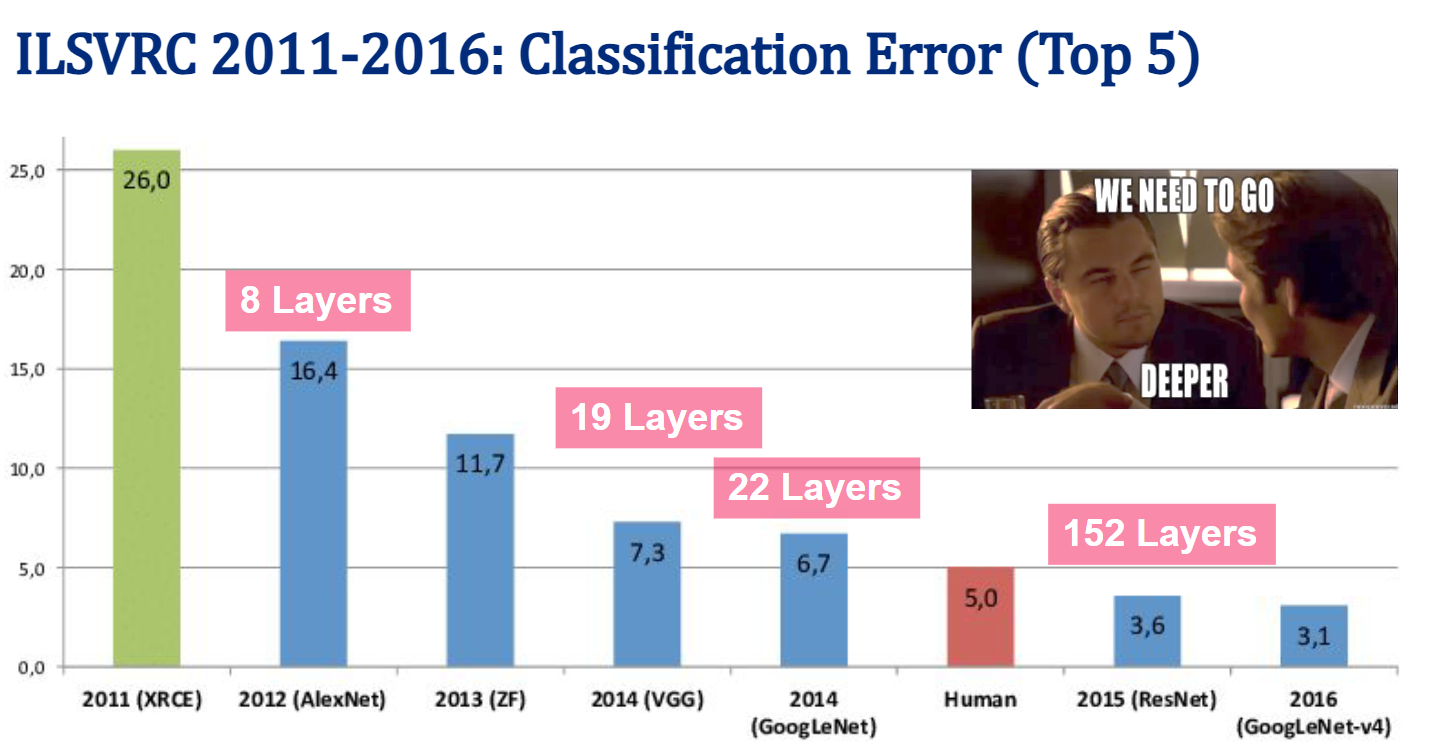
\includegraphics[width=0.5\linewidth]{modelsranked.png}
    \caption{ILSVRC Models Ranked}
    \label{fig:enter-label}
\end{figure}

\textbf{Post-ILVRC}
\begin{itemize}
    \item The last ILVRC competition was held in 2017
    \item ResNets are still the most popular architecture for a wide variety of problems
    \item Object recognition in-the-wild is still not solved
    \begin{itemize}
        \item Not all edge cases can be recognized yet
    \end{itemize}
\end{itemize}


\section{Transfer Learning}
\begin{definition}
    \textbf{Transfer Learning:} approach where a model trained on one task is re-purposed or fine-tuned for a different but related task. This leverages knowledge gained from the source task to improve learning efficiency and performance on the target task, particularly when data is limited.
\end{definition}

Generally, CNN models contain two distinct parts:

\begin{itemize}
    \item \textbf{Convolutional Layers} → Learn filters across spatial and channel dimensions \textbf{(encoder)}
    \item \textbf{Fully-connected Layers} → Learn to classify images based on the learned visual features \textbf{(classifier)}
\end{itemize}

The point at which these parts intersect is an \textbf{embedding}, which is a learned lower-dimensional set of "visual feature" representing the image. This embedding encodes everything needed from the image to classify objects! \\
This means that\textbf{ everything before the embedding is a general feature extraction that is universal} and can be applied to any model. The only specialized part of the model is the classifier, since it is unique to each problem. 

\begin{idea}
    The larger the encoder, the more universal it is. 
\end{idea}

\begin{definition}
    \textbf{Embeddings:} the process of representing objects, such as words, images, or entities, in a lower-dimensional space where their relationships and characteristics are preserved. These representations capture semantic or contextual information, making them suitable for various tasks like similarity measurement, classification, and recommendation.
\end{definition}

\begin{itemize}
    \item These CNN embeddings have proven useful for solving a wide variety of image-based problems
    \item By being trained on a large image classification dataset, CNNs learn something general about representing images!
\end{itemize}

We can use these features to transfer our learning to a new problem:
\begin{enumerate}
    \item Train CNN (e.g. AlexNet) on large image dataset (e.g. ImageNet)
    \item Remove "classification" layers at end of model, freeze remaining weights.
    \item Add, and train, new layers at end of model suitable for our new task.
\end{enumerate}

\begin{figure}[h!t]
    \centering
    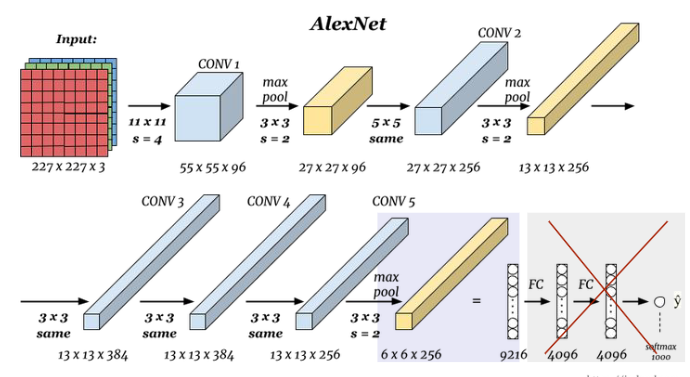
\includegraphics[width=0.45\linewidth]{transferlearning.png}
    \caption{Transfer Learning with AlexNet}
    \label{fig:enter-label}
\end{figure}

\begin{itemize}
    \item We froze the original model's weights, and used our CNN layers as a feature extractor
    \item Often training some/all of the original model's weights on the new task at a lower learning rate helps the features "adapt" to the new task
    \item This, and variants of it, is often referred to as \textbf{fine-tuning}

\end{itemize}

\begin{idea}
    \textbf{Transfer learning also prevents overfitting} because the architectures and weights of networks like AlexNet were trained using a larger dataset of over a million images, and were trained to solve a different image classification problem. Nevertheless, transfer learning allows us to leverage information from larger data sets with low computational cost. Effectively acting like a larger training set.
\end{idea}